\section{Simulation Results}

\begin{frame}{Simulation Results}
    \begin{block}{UAV Characteristics}
        \begin{itemize}
            \item 8 MP Digital camera;
            \item average speed: \SI{33}{mph};
            \item \SI{20}{frames/sec};\footnote{1200 frames per minute}
            \item UAV must be equipped with flash lights;
        \end{itemize}
    \end{block}
\end{frame}

\begin{frame}{Simulation Results}
    \begin{itemize}
        \item {\itshape improfile:} find the intensity profile of an image along a line segment.\footnote{Works with grayscale and RGB.}
    \end{itemize}

    \vfill

    \begin{columns}
        \begin{column}{0.45\textwidth}
            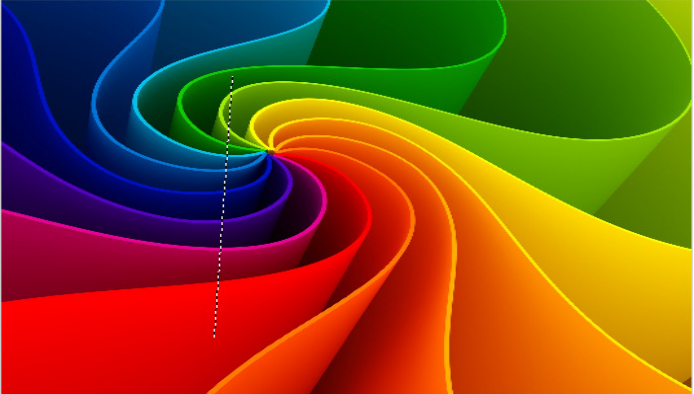
\includegraphics[width=\columnwidth]{figures/improfile1.png}
        \end{column}
        \hfill
        \begin{column}{0.45\textwidth}
            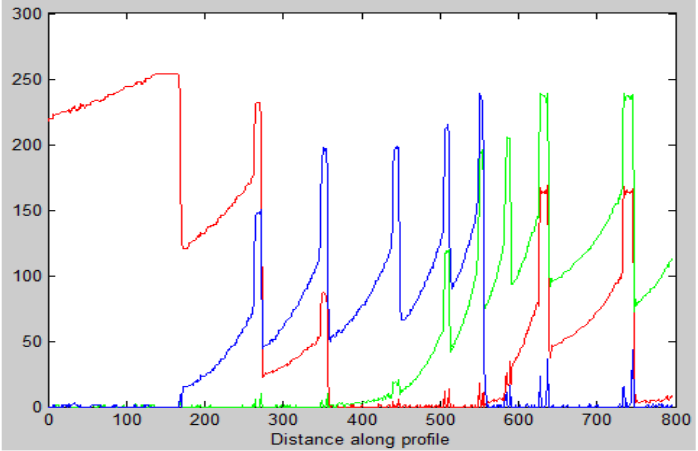
\includegraphics[width=0.95\columnwidth]{figures/improfile2.png}
        \end{column}
    \end{columns}
\end{frame}

% -----------------------------------------------------------------------------

\begin{frame}{Simulation Results}
    For crack detection in a railway track:

    \vfill
    
    \centering
    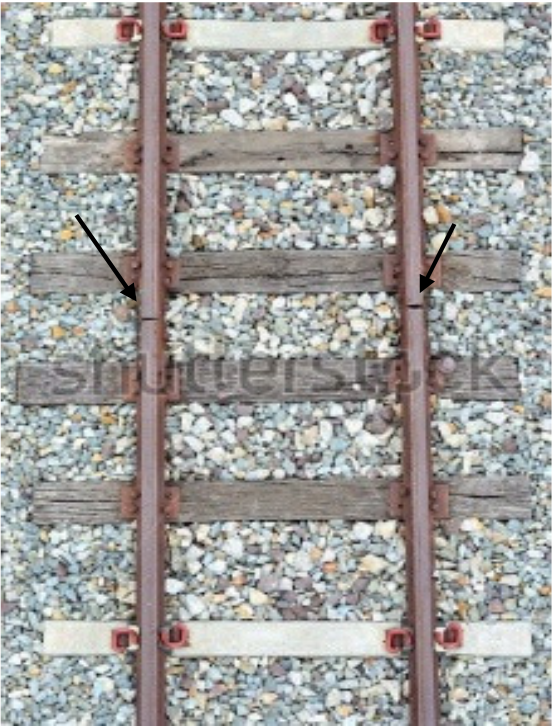
\includegraphics[scale=0.3, angle=90]{figures/railway1.png}
\end{frame}

% -----------------------------------------------------------------------------

\begin{frame}{Simulation Results}
    
    \begin{columns}
        \begin{column}{0.45\textwidth}
            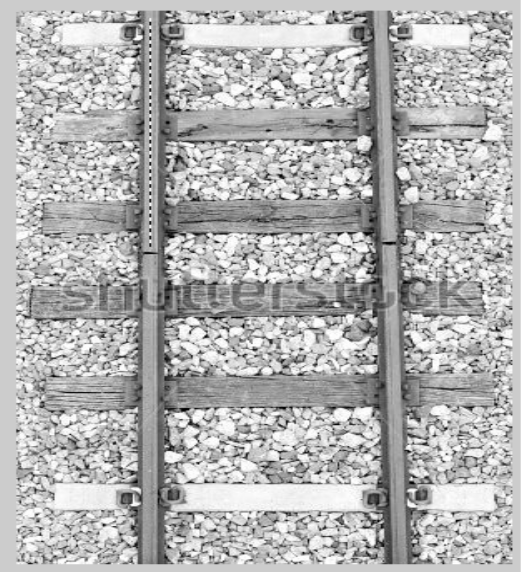
\includegraphics[width=\columnwidth]{figures/railway2.png}
        \end{column}
        \hfill
        \begin{column}{0.45\textwidth}
            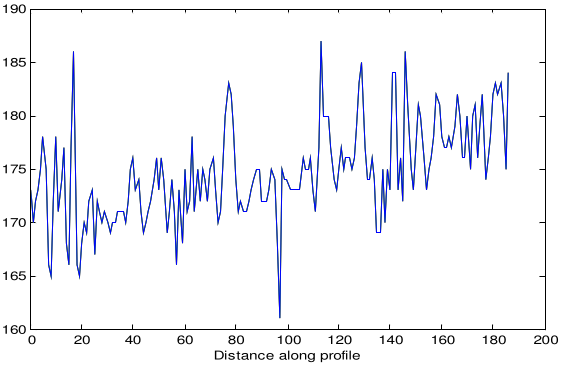
\includegraphics[width=\columnwidth]{figures/railway3.png}
        \end{column}
    \end{columns}

\end{frame}

% -----------------------------------------------------------------------------

\begin{frame}{Simulation Results}
    
    \begin{columns}
        \begin{column}{0.45\textwidth}
            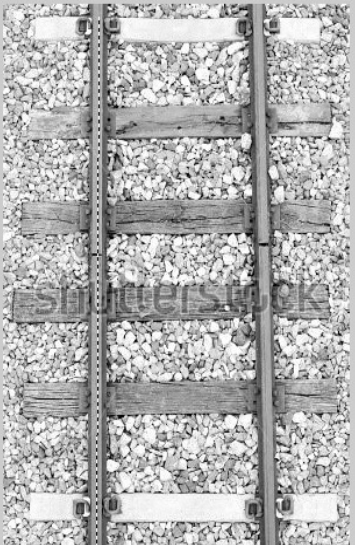
\includegraphics[width=0.75\columnwidth]{figures/railway4.png}
        \end{column}
        \hfill
        \begin{column}{0.45\textwidth}
            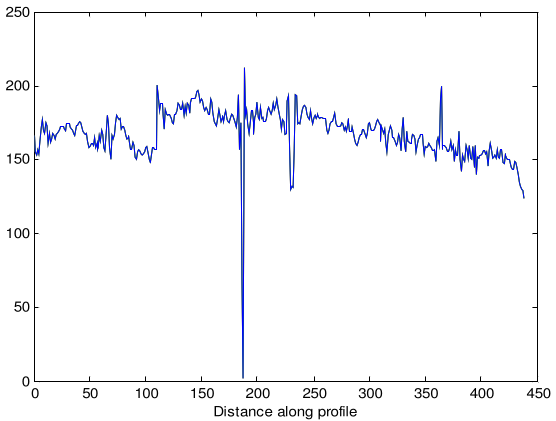
\includegraphics[width=\columnwidth]{figures/railway5.png}
        \end{column}
    \end{columns}

\end{frame}